
%(BEGIN_QUESTION)
% Copyright 2010, Tony R. Kuphaldt, released under the Creative Commons Attribution License (v 1.0)
% This means you may do almost anything with this work of mine, so long as you give me proper credit

Suppose we have an Allen-Bradley model ``SLC 500'' PLC connected to a liquid level switch, a selector switch, and a motor contactor (for a pump) as shown in this illustration:

$$\includegraphics[width=15.5cm]{i04634x01.eps}$$

Explain what conditions must be met for the pump to turn on, based on an analysis of the program running in the PLC:

$$\includegraphics[width=15.5cm]{i04634x02.eps}$$

\vskip 20pt \vbox{\hrule \hbox{\strut \vrule{} {\bf Suggestions for Socratic discussion} \vrule} \hrule}

\begin{itemize}
\item{} What condition(s) will cause the ``EN'' bit in timer {\tt T4:3} to activate?
\item{} How will this system behave if the contactor coil fails open?
\item{} How will this system behave if the contactor coil fails shorted?
\item{} How will this system behave if the level switch fails open?
\item{} How will this system behave if the wire connecting L1 to the VAC 1 terminal fails open?
\item{} How will this system behave if the wire connecting L2/N to the COM terminals fails open?
\end{itemize}

\underbar{file i04634}
%(END_QUESTION)





%(BEGIN_ANSWER)

The liquid level must exceed 5 feet in height for at least 25 seconds {\bf and} the selector switch must be in the ``right'' position in order for the pump to turn on.

%(END_ANSWER)





%(BEGIN_NOTES)









\vskip 20pt \vbox{\hrule \hbox{\strut \vrule{} {\bf Virtual Troubleshooting} \vrule} \hrule}

This question is a good candidate for a ``Virtual Troubleshooting'' exercise.  Presenting the diagram to students, you first imagine in your own mind a particular fault in the system.  Then, you present one or more symptoms of that fault (something noticeable by an operator or other user of the system).  Students then propose various diagnostic tests to perform on this system to identify the nature and location of the fault, as though they were technicians trying to troubleshoot the problem.  Your job is to tell them what the result(s) would be for each of the proposed diagnostic tests, documenting those results where all the students can see.

During and after the exercise, it is good to ask students follow-up questions such as:

\begin{itemize}
\item{} What does the result of the last diagnostic test tell you about the fault?
\item{} Suppose the results of the last diagnostic test were different.  What then would that result tell you about the fault?
\item{} Is the last diagnostic test the best one we could do?
\item{} What would be the ideal order of tests, to diagnose the problem in as few steps as possible?
\end{itemize}


%INDEX% PLC, relating I/O status to virtual elements

%(END_NOTES)


